%!TEX root = main.tex

\section{Secant Methods}
Both Newton-Raphson and Steepest descent are sound methods to compute local extrema of real-valued functions $f \colon \field{R}^d \to \field{R}$, with their pros and their cons.  
\begin{itemize}
	\item The method of Steepest descent always converges to a local minimum, yet slowly.  In order to obtain new approximations, we have to solve many different one-dimensional optimizations, each of them offering their own computational issues. 
	\item Newton offers faster sequences, but we cannot always guarantee convergence.  Another drawback of this method is the fact that we do need expressions for function itself, its gradient and Hessian matrix.  
\end{itemize}
In this section we are going to see a different concept based on the so-called \emph{secant method}, which will allow us to craft algorithms without those shortcomings.

\subsection{A secant method to search for roots of univariate functions}
To explain how it works, let's once again try to find an accurate value of $\sqrt{2}$ as the root of the polynomial $p(x) = x^2-2$.
\begin{enumerate}
	\item Consider two initial guesses $x_0=3$, $x_1=2.8$.  Notice $f(3)= 7 \neq 5.84 = f(2.8)$.
	\item The line that joins the points $(3, 7)$ and $( 2,8, 5.84)$ has equation
	\begin{align*}
	y - 7 &= \frac{5.84-7}{2.8-3}(x-3), \\ 
	y &= 5.8x-10.4.
	\end{align*}
	The latter can be seen as a linear approximation to the original function---one that did not use the derivative of $f$. This linear function intersects the $x$--axis at
	\begin{equation*}
	x_2 = \frac{10.4}{5.8} \approx 1.7931034483
	\end{equation*}
	We take this value as an approximation to the root of $f(x)=0$.
	\item Repeat this process to get a sequence of approximations $x_n$.
\end{enumerate}
\begin{example}
Observe the result of applying this recursive process, and compare with the similar experiment we conducted using the Newton-Raphson method in page \pageref{table:Newton-Raphson}.
\begin{center}
\begin{tabular}{|r|r|r|} \hline
$n$ & $x_n$ & $f(x_n)$ \\ \hline \hline
$0$ & $3.000000000000000$ & $7.0000E+00$ \\ \hline
$1$ & $2.800000000000000$ & $5.8400E+00$ \\ \hline
$2$ & $1.793103448275862$ & $1.2152E+00$ \\ \hline
$3$ & $1.528528528528528$ & $3.3640E-01$ \\ \hline
$4$ & $1.427253172054743$ & $3.7052E-02$ \\ \hline
$5$ & $1.414717869757887$ & $1.4267E-03$ \\ \hline
$6$ & $1.414215876250105$ & $6.5446E-06$ \\ \hline
$7$ & $1.414213562785585$ & $1.1667E-09$ \\ \hline
$8$ & $1.414213562373095$ & $8.8818E-16$ \\ \hline
\end{tabular}
\end{center}
\begin{figure}[ht!]
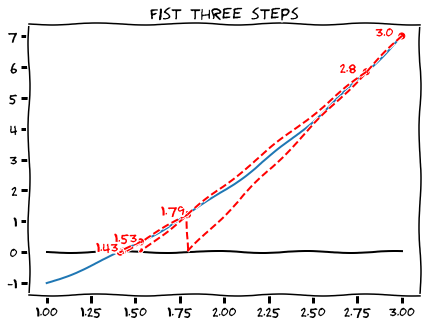
\includegraphics[width=0.6\linewidth]{images/secant.png}
\caption{Secant iterative method}\label{figure:SecantMethod}
\end{figure}
\end{example}

\begin{definition}\label{def:SecantMethod}\index{Secant method}\index{Secant method!iteration}\index{Secant method!recursive formula}
Given a function $f \colon \field{R} \to \field{R}$ and two initial guesses $x_0 \neq x_1$ satisfying $f(x_0) \neq f(x_1)$, we define the \emph{Secant method iteration} to be the sequence $\{ x_n \}_{n \in \field{N}}$ obtained by one of the following recursive formulas:
\begin{equation}\label{equation:SecantMethod}\index{Secant method!iteration}
\begin{split}
\bigg[\frac{f(x_n) - f(x_{n-1})}{x_n - x_{n-1}}\bigg] (x_{n+1} - x_n) = - f(x_n) \\
x_{n+1} = x_n - \bigg[ \frac{x_n - x_{n-1}}{f(x_n) - f(x_{n-1})} \bigg] f(x_n)
\end{split}
\end{equation}
The \emph{Secant method} refers to employing this sequence to search and approximate roots of the equation $f(x)=0$.
\end{definition}

\subsection{Efficiency of the Secant Method}
Let $f \colon \field{R} \to \field{R}$ be a real-valued function with a root $x^\star$, and let $\{ x_n \}_{n \in \field{N}}$ be a secant method iteration.  
\begin{align*}
x_{n+1} - x^\star &= x_n - \frac{x_n - x_{n-1}}{f(x_n) - f(x_{n-1})} f(x_n) - x^\star \\
&= (x_n - x^\star) \bigg( 1 - \frac{x_n - x_{n-1}}{f(x_n) - f(x_{n-1})}  \frac{f(x_n) - \overbrace{f(x^\star)}^0}{x_n - x^\star} \bigg) \\
&= (x_n - x^\star) \bigg(  1 - \frac{\Delta f [x_n, x^\star]}{\Delta f [x_{n-1}, x_n]} \bigg) \\
&= (x_n - x^\star) \frac{\Delta f [x_{n-1}, x_n] - \Delta f [x_n, x^\star]}{\Delta f [x_{n-1}, x_n]} \\
&= (x_n - x^\star) \frac{\Delta f [x_{n-1}, x_n] - \Delta f [x_n, x^\star]}{x_{n-1}-x^\star} \frac{x_{n-1}-x^\star}{\Delta f [x_{n-1}, x_n]} \\
&= (x_n - x^\star) (x_{n-1} - x^\star) \frac{\Delta f [x_{n-1}, x_n, x^\star]}{\Delta f [x_{n-1}, x_n]}
\end{align*}

We use this identity to prove the corresponding \emph{local convergence result}, as we did for the Newton-Raphson method:

\begin{theorem}[Local Convergence for the Secant Method]\label{theorem:LCScnt}\index{Secant method!Local convergence for}\index{Theorem!Local Convergence for Secant}
Let $x^\star$ be a simple root of the equation $f(x)=0$, and there exists $\varepsilon > 0$ so that 
\begin{itemize}
	\item $f$ is twice continuously differentiable in the interval $(x^\star-\varepsilon, x^\star + \varepsilon)$, and
	\item there are no critical points of $f$ on that interval.
\end{itemize}  
Set
\begin{equation*}
M(\varepsilon) = \max \bigg\{ \bigg\lvert \frac{f''(s)}{2f'(t)} \bigg\rvert : x^\star -\varepsilon < s,t < x^\star + \varepsilon \bigg\}.
\end{equation*}
If $\varepsilon$ is small enough so that $\varepsilon M(\varepsilon) < 1$, then
\begin{enumerate}
	\item \label{thm:LCScnt1} There are no other roots of $f$ in $(x^\star -\varepsilon, x^\star+\varepsilon)$.
	\item \label{thm:LCScnt2} Any Secant method iteration starting with initial guesses $x_0 \neq x_1$ (none of them equal to $x^\star$, and with $f(x_0) \neq f(x_1)$) in that interval will converge (quadratically) to $x^\star$
\end{enumerate} 
\end{theorem}

The proof is similar to the one for Theorem \ref{theorem:LCNR}, and is left as exercise.

\subsection{Generalization of the Secant Method to higher dimensions: Broyden's Method}
The objective now is the search of a root for a function $\boldsymbol{g} \colon \field{R}^d \to \field{R}^d$, which we assume of the form 
\begin{equation*}
\boldsymbol{g}(x_1, \dotsc, x_d) = \big[ g_1(x_1, \dotsc, x_d), \dotsc, g_d(x_1, \dotsc, x_d) \big]
\end{equation*}
for appropriate functions $g_k \colon \field{R}^d \to \field{R}$ ($1 \leq k \leq d$).  We start at an initial guess $\x_0 \in \field{R}^d$ and, if possible, we choose as $\x_1$ the first step of Newton-Raphson: 
\begin{equation*}
\transpose{\x_1} = \transpose{\x_0} - \big[ \gradient{\boldsymbol{g}}(\x_0) \big]^{-1} \cdot \transpose{\boldsymbol{g}(\x_0)}
\end{equation*}
At that point we craft a linear approximation $\boldsymbol{L}_1 \colon \field{R}^d \to \field{R}^d$ to the graph of $\boldsymbol{g}$ that interpolates $\big( \x_0, \boldsymbol{g}(\x_0) \big)$ and $\big( \x_1, \boldsymbol{g}(\x_1) \big)$.  We may impose this \emph{secant property} by requesting $\boldsymbol{L}_1$ to be of the form\index{Secant property}
\begin{equation*}
\transpose{\boldsymbol{L}_1(\x)} = \transpose{\boldsymbol{g}(\x_1)} + \boldsymbol{A}_1 \cdot \transpose{(\x - \x_1)},
\end{equation*}
where $\boldsymbol{A}_1$ is a non-singular square matrix of size $d \times d$ that satisfies
\begin{equation*}
\boldsymbol{A}_1 \cdot \transpose{(\x_1 - \x_0)} = \transpose{\boldsymbol{g}(\x_1)} - \transpose{\boldsymbol{g}(\x_0)}.
\end{equation*}
At this point, we approximate the root of $\boldsymbol{g}$ by the root $\x_2$ of $\boldsymbol{L}_1$:
\begin{equation*}
\boldsymbol{A}_1 \cdot \transpose{(\x_2 - \x_1)} = -\transpose{\boldsymbol{g}(\x_1)},
\end{equation*}
or equivalently,
\begin{equation*}
\transpose{\x_2} = \transpose{\x_1} - \boldsymbol{A}_1^{-1} \cdot \transpose{\boldsymbol{g}(\x_1)}.
\end{equation*}
We repeat this process to obtain a sequence of approximations $\{ \x_n \}_{n \in \field{N}}$ via a sequence of non-singular square matrices $\boldsymbol{A}_n$ of size $d \times d$ that satisfy the secant property
\begin{equation}\label{equation:SecantProperty}
\boldsymbol{A}_n \cdot \transpose{(\x_{n+1} - \x_n)} = \transpose{\boldsymbol{g}(\x_{n+1})} - \transpose{\boldsymbol{g}(\x_n)}.
\end{equation}
The corresponding linear functions are given by 
\begin{equation*}
\transpose{\boldsymbol{L}_n (\x)} = \transpose{\boldsymbol{g}(\x_n)} + \boldsymbol{A}_n \cdot \transpose{(\x - \x_n)}.
\end{equation*}
The recurrence formula can be expressed in any of the following two ways:
\begin{equation}
\begin{split}
\boldsymbol{A}_n \cdot \transpose{(\x_{n+1} - \x_n )} = -\transpose{\boldsymbol{g}(\x_n)}, \\
\transpose{\x_{n+1}} = \transpose{\x_n} - \boldsymbol{A}_n^{-1} \cdot \transpose{\boldsymbol{g}(\x_n)}
\end{split}
\end{equation}

There is not a unique way to choose these matrices $\boldsymbol{A}_n$ (and I encourage you to find one of your own devise).  A straightforward method is given by the following recursive formulas:
\begin{align}\index{Broyden Method!recursive formula}\index{Broyden Method!iteration}
\boldsymbol{A}_0 &= \gradient{\boldsymbol{g}}(\x_0) \nonumber \\
\boldsymbol{A}_{n+1} &= \boldsymbol{A}_n + \frac{\big[ (\boldsymbol{g}(\x_n)-\boldsymbol{g}(\x_n)\big) - \boldsymbol{A}_n (\x_{n+1}-\x_n) \big] \otimes (\x_{n+1} -\x_n)}{\norm{\x_{n+1}-\x_n}^2} \label{equation:Broyden}
\end{align}
We refer to this process as the \emph{Broyden Method} for finding roots.\index{Broyden Method}

\begin{example}
Let's use this method to find any of the roots $(-1,-1)$, $(0,0)$, $(1,1)$ of the function $\boldsymbol{g}(x,y) = \big[ x^3-y, y^3 - x \big]$ from Example \ref{example:preNewton4poly4}.
Starting with initial guess $(x_0, y_0) = (-1, 1)$, we take the first step from Newton-Raphson:
\begin{align*}
\gradient{\boldsymbol{g}}(x_0, y_0) &= \begin{bmatrix} 3x_0^2 & -1 \\ -1 & 3y_0^2 \end{bmatrix} =  \begin{bmatrix} 3 & -1 \\ -1 & 3 \end{bmatrix} \\
\transpose{\boldsymbol{L}_0 (x, y)} &= \begin{bmatrix} -2 \\ 2 \end{bmatrix} + \begin{bmatrix} 3 & -1 \\ -1 & 3 \end{bmatrix} \cdot \begin{bmatrix} x \\ y \end{bmatrix} = \begin{bmatrix} 3x -y -2 \\ -x+3y +2 \end{bmatrix}
\end{align*}
This gives $(x_1, y_1) = (-1/2, 1/2)$ as root of $\boldsymbol{L}_0$.  For the second step, we compute the matrix $\boldsymbol{A}_1$ satisfying the secant property:
\begin{align*}
\boldsymbol{A}_1 &= \begin{bmatrix} 3 & -1 \\ -1 & 3 \end{bmatrix} + 2 \big( \big[ -\tfrac{5}{8}, \tfrac{5}{8} \big] \otimes \big[ \tfrac{1}{2}, -\tfrac{1}{2} \big] \big) \\
&= \begin{bmatrix} 3 & -1 \\ -1 & 3 \end{bmatrix} + 2 \begin{bmatrix} -\tfrac{5}{8} \cdot \tfrac{1}{2} & -\tfrac{5}{8}\cdot \big( -\tfrac{1}{2} \big) \\ \tfrac{5}{8} \cdot \tfrac{1}{2} & \tfrac{5}{8} \cdot \big(- \tfrac{1}{2} \big) \end{bmatrix} \\
&= \begin{bmatrix} 3 & -1 \\ -1 & 3 \end{bmatrix} + \begin{bmatrix} -5/8 & 5/8 \\ 5/8 & -5/8 \end{bmatrix} = \begin{bmatrix} 19/8 & -3/8 \\ -3/8 & 19/8 \end{bmatrix}
\end{align*}
This gives a linear approximation 
\begin{align*}
\transpose{\boldsymbol{L}_1(x,y)} &= \begin{bmatrix} -5/8 \\ 5/8 \end{bmatrix} + \begin{bmatrix} 19/8 & -3/8 \\ -3/8 & 19/8 \end{bmatrix} \cdot \begin{bmatrix} x + 1/2 \\ y - 1/2 \end{bmatrix} \\
&= \begin{bmatrix} \tfrac{19}{8}x-\tfrac{3}{8}x + \tfrac{3}{4} \\ \\ -\tfrac{3}{8}x+\tfrac{19}{8}y - \tfrac{3}{4} \end{bmatrix}
\end{align*}
which has root $(x_2, y_2) = (-3/11, 3/11)$.
\end{example}